\documentclass[conference]{IEEEtran}
\usepackage{amssymb}
\usepackage{amsmath}
\usepackage{graphicx}
\usepackage{wasysym}
\usepackage{siunitx}
\usepackage{tabularx, booktabs}
\usepackage[draft]{hyperref}
\hyphenation{op-tical net-works semi-conduc-tor}

\DeclareMathOperator*{\argmax}{\arg\!\max}
\DeclareMathOperator*{\softmax}{\texttt{softmax}}

\begin{document}

\renewcommand{\figureautorefname}{Fig.}
\newcommand{\subfigureautorefname}{Fig.}
\renewcommand{\sectionautorefname}{Section}
\renewcommand{\subsectionautorefname}{Section}


\title{EEL6935 Course Project Final Report \\
    Sentiment Analysis}
\author{\IEEEauthorblockN{
    Caleb Bryant\IEEEauthorrefmark{1},
    Jixin Feng\IEEEauthorrefmark{2}}
\IEEEauthorblockA{Department of \\
    \IEEEauthorrefmark{1} Computer \& Information Science \& Engineering\\
    \IEEEauthorrefmark{2} Electrical \& Computer Engineering\\
    University of Florida,
    Gainesville, FL, 32611\\
    Email: \texttt{{\small\{cal2u,fengjixin\}}@ufl.edu}}}

\maketitle

\begin{abstract}
    The volume of text on the Internet -- unstructured text especially --
    is increasing with drastic speed everyday. Unlike human brains, traditional 
    computer programs have a much more limited ability to extract useful
    information from unstructured text with satisfactory precision.
    While traditional machine learning methods have had some success
    tackling NLP problems with ``bag of words'' models and feature engineering,
    deep learning and the subsequent development of robust word embeddings have shown
    promising results and have made substantial ground towards replacing older methods.
    In this course project for EEL6935 Big Data Ecosystems, we implemented a sentence 
    classification program for sentiment analysis based on Long-Short Term Memory Network 
    (LSTM) and compare the performance with a logistic regression based baseline model. 
    In addition, we also created a web application able to do real-time sentiment analysis
    based on the model we created. 
    
\end{abstract}

\IEEEpeerreviewmaketitle

\section{Introduction}
\label{intro}
    With the tremendous volume of unstructured text generated everyday, both on and off
    the internet, the amount of attention devoted to processing and extracting useful information
    from it has been constantly increasing. It is predicted that by 2020 the
    total data volume of the ``digital universe'' will increase to 40 ZB
    ($40\times 10^{21}$ bytes), which is about 50 times larger than that is was in
    year 2010\cite{gantz2012digital}. Most of the text will be generated by
    sources like the news media, social networks, medical facilities, etc.

    Although this text data is a valuable source of information
    and can be easily comprehended by humans, current computational methods
    continue to struggle extracting information from unstructured text 
    sources.
    Hence effective methods to process and analyze unstructured text data are
    desperately needed.

    In this course project, we are targeting a specific domain of text analysis
    problems -- sentiment analysis. The goal of sentiment analysis is to assign
    proper pre-defined sentiment labels to a given text, so that the emotion behind the
    sentence can be represented and then categorized\cite{allahyari2017brief}.
    Mathematically, the classification model can be represented as:
    $$f:\mathcal{D}\rightarrow\mathcal{L}$$
    w $\mathcal{D}=\{d_0, d_1,\ldots, d_{n-1}\}$ is the set of sentences
    , and $\mathcal{L}=\{l_0, l_1,\ldots, l_{k-1}\}$ is the set of labels.
    Depending on whether multiple labels are allowed to be assigned to a document, the
    classification is called soft or hard\cite{gopal2010multilabel}. When conducting sentiment 
    analysis, the set of labels is usually binary, and they can be used
    to model the overall opinion the subject received. Movie reviews, for example,
    can be labeled as positive or negative\cite{pang2002thumbs}.

    In cases w t is an uneven class distribution, the performance
    of a sentiment analysis system can be evaluated with its
    F-1 score, which can be defined as\cite{forman2003extensive}:
    $$F_1=\frac{2}{\frac{1}{r}+\frac{1}{p}}=\frac{2pr}{p+r}$$
    w $p=\frac{tpr}{tpr+fpr}$ stands for precision and $r=\frac{tpr}{tpr+fnr}$
    stands for recall.

    Historically, sentiment analysis has been done via statistical
    and machine learning methods like Naive Bayes, k-nearest neighbors, decision
    trees, SVM, and so on. In this report, we decide to compare the performance of
    sentence classifier based on different techniques: 
    classic Bag-of-Words\cite{pang2002thumbs},
    Convolutional Neural Network (CNN)\cite{kim2014convolutional} 
    and Long Short-Term Memory (LSTM)\cite{barnes2017assessing}.
    
    We divided our project into two stages: the back-end of sentiment analysis
    and a web-based front-end. The backend program is designed to implement 
    LSTM and compare its performance with the Logistic Regression as a baseline
    of performance. The front-end web application is build with Flask, a 
    a micro web development framework for Python.
    
    The dataset we used to train the system is Stanford Large Movie Review 
    Dataset\cite{maas2011learning}. It's a data set with 25,000 highly polarized
    movie reviews for training purpose and another 25,000 reviews for testing.
    Both raw text and bag-of-words formats of data are included in this dataset
    
    The report is organized as follows: 
    A brief introduction of related research contribution is in \autoref{related}.
    system architecture and different analysis approaches are introduced and compared 
    in \autoref{model}.
    The benchmarks used for evaluating the performance and our simulation environment, 
    dataset, simulation result are presented in \autoref{performance}.
    The conclusion and the source code of our program, report and 
    presentation in \LaTeX, as well as the web-application are introduced in 
    \autoref{conclusion}.
    The team coordination is introduced in \autoref{team}.
    
\section{Related Work}
\label{related}
\subsection{Early Research}
    Sentiment analysis has been actively studied for a long time. At the very beginning
    of its research, classifying sentiment of a document is still a very challenging
    task, so earlier research are mostly focus on classifying document based on their 
    publisher, style, etc.\cite{biber1991variation}. Later in the 90s, researchers 
    were able to classify the genre 
    of text\cite{karlgren1994recognizing,kessler1997automatic}, 
    which is one step closer to the sentiment of the text
    than merely publisher and style of the text. Detecting whether
    the text includes a subjective opinion was not generally possible until early 
    2000s\cite{hatzivassiloglou2000effects}. This marks the beginning of 
    sentiment analysis. Most of the early attempts try to  classify by detecting 
    the sentiment of the entire piece of text\cite{pang2002thumbs,pang2005seeing}. 
    This is relatively easy to achieve but may lost track of the detailed sentiment
    or mixed sentiment\cite{lu2011multi}.
    With the help of significantly improved
    computation power of CPU and GPUs, neural network related techniques 
    started to show great potential in the sentiment analysis 
    domain\cite{kim2014convolutional,barnes2017assessing}.

\subsection{Application in Business Domain}
    Sentiment analysis on reviews has huge application potential. In the domain of 
    shopping for example, more and more consumers nowadays are making 
    purchase decisions about a product not only based on the self introduction of the 
    product but the reputation summarized by the review of it. And the research
    shows that online review of a product can even affect the off-line shopping
    behavior\cite{lipsman2007online}. According to a survey of more than 2000 
    American adults, more than 80\% of internet users (about 60\% of American) 
    does online research before making an off-line purchase at least once per year.
    And among all the online reviews read by internet users, about 73\% to 87\% reviews
    have significant influence on purchasing behaviors especially in the domain
    of restaurant and hotel\cite{pang2008opinion}.
    
    Because online reviews possess such great potential of influence of purchasing
    behavior. The vendors are showing increasing amount of interests of studying them
    too. A white paper published back in 2006\cite{kim2006forrester} shows that 
    there were estimated 75,000 blogs and 1.2 million online posts generated 
    everyday, and that was more than 10 years ago. A blog post published by twitter
    in 2013 shows that the average TPS (tweets per second) was 5,700 and the record
    of 143,199 TPS was created on Aug. 16 2013\cite{tps2013}. With such big number of
    new text generated everyday, any small disturbance of public opinion on any subject
    may bring significant impact on people's behavior.
    
    With the evolvement of online media streaming service, reviews generated from
    from watching movie and online media has become one of the major component of 
    online review. A press release by YouTube claims that with more than 1 billion
    users from 88 countries and speaking 76 languages, there are 1 billion
    hours of YouTube Video has been watched daily. These users' rate and review of 
    video content can be a good source for business decision making. 
    
    Sentiment analysis of movie reviews is a domain with experimentally conveniency
    because most dataset of movie review gathered already associated with indicators 
    can be easily extracted and processed by computer program such as
    ``Like'' or five-star-rating. The accuracy of those indicators are usually sufficiently
    high, so a numerous of time of manually labelling those data can be saved. But
    according to previous research\cite{turney2002unsupervised}, movie reviews are
    considered one of most difficult domains for sentiment analysis. Early research
    on movie reviews hardly get accuracy much better than random outcome 
    (50\% accuracy) even in simple binary classification case\cite{pang2002thumbs}.
    So a good research of sentiment analysis on movie reviews is in need.
    
\section{System Architecture}
\label{model}
\subsection{Representation and Encoding of Text}
\label{model:represent}
    Text documents, in its original form, can not be easily processed
    by computer programs. And the data structure used to represent them usually plays 
    an important role in text processing\cite{hotho2005brief,allahyari2017brief}. Hence
    Text preprocessing and encoding should be handled carefully.
    
\subsubsection{Text Preprocessing}
\label{model:represent:preprocess}
    Previous research has shown that preprocessing of text is able to product observable
    influence on the success of text classifications\cite{uysal2014impact}.
    Generally speaking, text preprocessing usually contains in 4 
    tasks\cite{allahyari2017brief}:
    \begin{itemize}
        \item Tokenization
        \item Filtering
        \item Lemmatization
        \item Stemming
    \end{itemize}
    
    The task of tokenization is to remove the unnecessary parts of the text like 
    punctuation marks and break the text into smaller building blocks like words and 
    phrases\cite{webster1992tokenization}. 
    Filtering is the task aims to remove the part of the text that convey close to zero 
    information. Example of such elements includes conjunctions and 
    prepositions\cite{silva2003importance}.
    Lemmatization and stemming share similar purpose: seeking the correlation between words.
    Lemmatization groups the words within same role of the text together so they can be 
    analyzed as one element. Stemming tries to find a root of text first and create the tree
    structure to represent the relationship between them\cite{hull1996stemming}.

\subsubsection{Text Encoding and Representation}
\label{model:represent:encoding}
    Computer programs will typically only treat text as an array of characters.
    But machine learning systems can only treat input and output data as numerical
    scalars or vectors. So in order to feed text to machine learning models, we need to 
    convert conventional text into mathematically representable forms. One of the most
    common method to encode text data to match the format requirement of machine
    learning algorithm is to convert them into numerical vectors. The approach is called
    ``Vector Space Model'' (VSM). VSM is widely used in the domain of text mining, and
    it offers great efficiency while processing large scale text data 
    sets\cite{salton1975vector,hotho2005brief}.
    
    In VSP representation of text, each word can be represented by a numerical value 
    used for encoding called the weight of the word. 
    One of the most straight forward text representation method is Bag-of-Words (BoW), 
    which simply keep track of the occurrence and frequency of each word/phrase of the text 
    while ignore the order of them, and produce a vector representation of text, which 
    basically means no preprocessing, only encoding. 
    This make the processing easier but lots of information can be lost in the 
    representation. 
    Words are treated as categorical data, and the programs do not put much consideration
    into the relations between them. While this creates simplicity, it means that all 
    words are treated as being equally different from one another, and this does not 
    align with humans' common understanding of language. 
    Movie review for example, ``I love the story but hate the music'', 
    and ``I love the music but hate the story'' may end up as same vector representation
    if BoW is implemented. Hence more comprehensive preprocessing and encoding techniques
    are need to be applied.
    Researchers in Google spent a lot of effort on this topic and 
    made quite noticeable contributions\cite{mikolov2013efficient, word2vec}.
    
    When written in mathematical terms, we can define the collection of text documents
    to be $$\mathcal{D}=\{d_1, d_2,\ldots,d_D\}$$, and
    let $$\mathcal{V}=\{v_0, v_1,\ldots, v_{m-1}\}$$ be an m-word predefined set called
    vocabulary. Each word in $\mathcal{V}$ will have a corresponding feature in
    machine learning model. The notation of frequency of a word $v\in\mathcal{V}$ occurred 
    in document $d\in\mathcal{D}$ is $f_d(v)$, hence a document can be represented as
    a vector $$\bar{d}=\{f_d(v_1),f_d(v_2),\ldots\}$$.
    And the notation of total number of documents
    $d\in\mathcal{D}$ containing the word $w$ is represented as $f_\mathcal{D}(v)$
    
    We can also use metrics other than the word frequency. Boolean weight, for example, 
    assigns 
    $$\omega_{ij} = \begin{cases} 
        1 & v_i \in d_j\\
        0 & v_i \notin d_j
    \end{cases}$$
    
    The Term Frequency-inverse Document Frequency (TF-IDF) is also a popular metric of
    word weighting metric. In this metric scheme, the weight of each word $v$ 
    in document $d$ can be calculated as:
    $$q(v)=f_d(v)\log\frac{\left|\mathcal{D}\right|}{f_\mathcal{D}(v)}$$
    
    Based on the weighting metric, a text/document can be represented by a vector 
    $$w(d)=(w(d,v_1),w(d,v_2),\ldots)$$,
    Hence the similarity between two documents $d_1$ and $d_2$ can be measured using 
    cosine similarity\cite{salton1988term}
    $$S(d_1,d_2)=\cos(\theta)=\frac{d_1d_2}{
    \sqrt{\sum_{i=1}^{\left|\mathcal{V}\right|}{v_{1i}^2}}
    \sqrt{\sum_{i=1}^{\left|\mathcal{V}\right|}{v_{2i}^2}}
    }$$

\subsection{Backend}
\label{model:back}
    In this course project, we want to implement a convolutional neural network
    model for text sentiment analysis, and compare its performance to baseline results
    generated by a bag-of-words model paired with a conventional machine learning
    technique, logistic regression.
    
\subsubsection{Logistic Regression}
\label{model:back:lr}
    Traditionally, sentiment analysis can be done by conventional machine learning
    methods such as Na\"ive Bayes, maximum entropy, logistic regression and 
    support vector machines (SVM). 
    To establish a baseline for our later work with Neural Networks, we have
    created a implemented a basic logistic regression model using tensorflow. Given a 
    dictionary of size $N$, each input $x_i$ is a $N \times 1$ dimension bag-of-words 
    encoding for the $i$-th sentence in our training set. Assuming that each $x_i$ 
    belongs to one of $C$ possible classes, $W$ is a $N \times C$ weight matrix, 
    and $b$ is a $C \times 1$ bias, our prediction $\hat{y}$ 
    is defined as follows\cite{ng2002discriminative,hosmer2013applied}:

    $$\hat{y} = \sigma(x^T_i W +b)$$
    $$\sigma (x)_{j}={\frac {e^{x_{j}}}{\sum _{i=1}^{N}e^{x_{i}}}}$$
    
    Note that the softmax function maps each dimension of its input to a value between 0
    and 1, and the transformation also normalizes the predicted probabilities such that
    they sum to 1 for multi-class prediction. Each entry $\hat{y}_i$ corresponds to 
    the predicted probability of the input sentence $x$ belonging to class $i$.
    \begin{figure}
        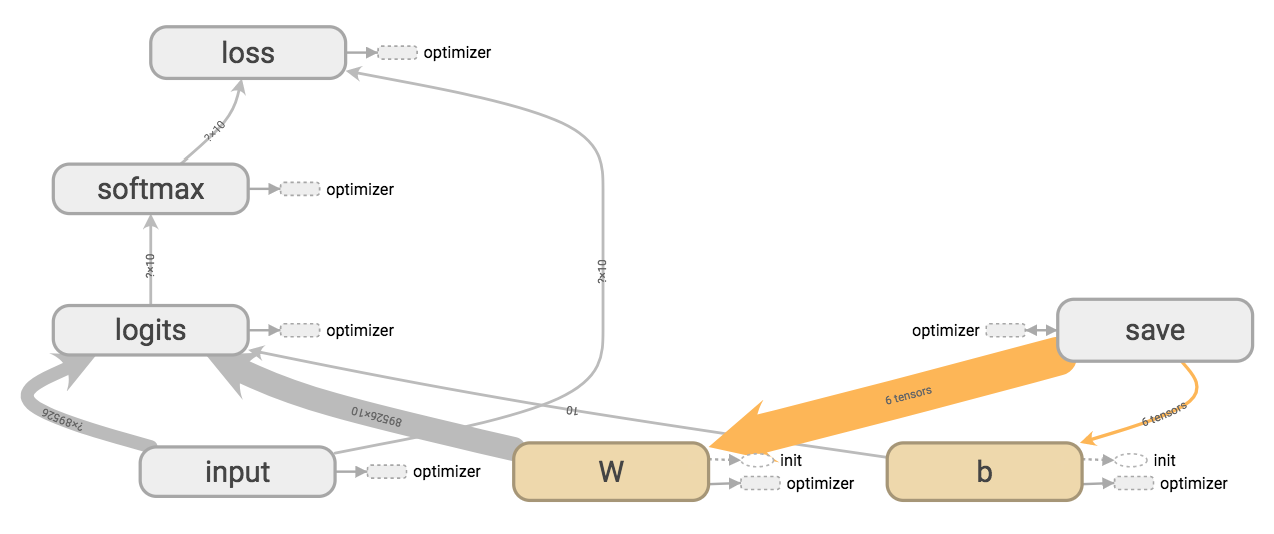
\includegraphics[width=0.45\textwidth]{figure/model_architecture}
        \caption{Our logistic regression architecture visualized with Tensorboard.}
    \end{figure}
    
    Since this model is both commonly used and simple to implement, it forms a good baseline
    for our future work. Our results for this model are reported later on in the document.

\subsubsection{Long Short-Term Memory (LSTM)}
\label{model:back:lstm}
    The LSTM model was originally proposed by Sepp Hochreiter and 
    J\"urgen Schmidhuber back in 1997\cite{hochreiter1997long} aiming to solve one
    of the biggest inherent flaw in previously proposed Recurrent Neural Networks (RNN).
    The conventional RNN implementation doesn't handles temporal propagation of 
    error signals very well, and in some cases, the error signals may propagate
    back in time domain with exponential growth or attenuation. Hence whatever the
    network tries to back-propagate, it either quickly blows up or vanished to the
    void\cite{gers1999learning}, which called the gradient vanishing.
    This problem stops standard RNN to learn anything from 
    the temporal points further than 5-10 steps away, and making people doubt the real
    potential of RNN on time-window-based learning systems. LSTM, on the other hand, is
    able to bridge information located in much longer time span.
    
    The original implementation of LSTM allows information across arbitrary time span
    to be stored in the cell, and same for the error signals. This enabled LSTM to 
    pick up the information with extraordinary lags between them but may also leads to 
    LSTM cell saturation, and fail to perform as memory cells. So the original LSTM 
    implementation requires periodically reset to keep operational. A mechanism called
    forget gate were proposed later to solve this problem\cite{gers1999learning}. This 
    allowed LSTM to learn continuously without reset.
    
    Since then, researchers start to propose various innovative LSTM modifications.
    Extended Karman Filter can be used for training the LSTM to solve some pathological
    learning cases\cite{perez2003kalman}. When implemented to operate on both temporal
    directions, LSTM then becomes Bidirectional LSTM 
    (Bi-LSTM)\cite{schuster1997bidirectional,barnes2017assessing}.
    If the input and the forget gate are merged into one update gate, the modified LSTM
    is then called Gated Recurrent Unit (GRU)\cite{cho2014learning}.
    
    Given a word sequence $S=\{v_0,v_1,\ldots,v_{l-1}\}$ with length $l$, the states
    of LSTM are updated as:
    $$
    \begin{bmatrix} 
    i_t\\f_t\\o_t\\c_t 
    \end{bmatrix} = 
    \begin{bmatrix}
    \sigma\\\sigma\\\sigma\\\tanh
    \end{bmatrix}
    S[h_{t-1},x_t]
    $$
    , in which $c_t=f_t\circ c_{t-1} + i_t\circ\hat{c_t}$ and $h_t=o_t\circ\tanh{c_t}$.
    At time $t$ in this relationship, $c_t$ and $h_t$ are the LSTM memory and 
    hidden state, $\hat{c_t}$ is the current cell state. The input at time $t$ 
    is $x_t$ and the input/forget/output gate activation are represented by $i$, 
    $f$ and $o$ respectively. $\sigma$ and $\circ$ are notations of logistic 
    sigmoid function and element-wise multiplication.\cite{zhou2016text}.
        
    To build our LSTM model, first we define a dictionary 
    $D = [w_1, w_2...w_N]$ 
    to contain the set of all words representable by our LSTM network. The $i$-th
    input to our LSTM is a vector
    $$
    v_i = [ \pi_{i1}, \pi_{i2}... \pi_{iL}]
    $$
    corresponding to a movie review $r_i$ of length $L$, where $\pi_{ij}$ is the dictionary index of 
    the $j$-th word of $r$. To see how this would work in practice, let 
    $D = [\text{cat}, \text{dog}, \text{meow}]$. Then the review 
    $r =  [\text{dog}, \text{dog}, \text{cat}, \text{meow}]$ would be encoded 
    $v = [1, 1, 0, 2]$, assuming a 0-indexed dictionary.
    
    In order to help the LSTM learn how to interpret the words in a movie review,
    each sentence's words are embedded inside a weight matrix $W_e$ with
    dimensions $N \times E$. The value $E$ is a hyperparameter known as the 
    embedding dimension and often ranges between 50 and 300. The rows of the
    embedding matrix are called word vectors, and approaches such as word2vec 
    \cite{word2vec} and GloVe \cite{pennington2014glove} can be used to learn 
    distributed embeddings for each word present in a corpus.
    
    After initializing the hidden state to zeros at the beginning of each batch, sequences
    of embeddings
    $$
    s_i = [ e_{i1}, e_{i2}, .. e_{iL}] 
    $$
    are then sequentially fed into the LSTM layer of our network, where each $e_{ij}$ is
    the embedding vector for the word $w_{ij}$, looked-up according to the input index
    $\pi_{ij}$. Only the final output state of the LSTM is used for prediction, and it is
    fed into a fully-connected softmax layer.
    
    In our model, we use pre-trained 100-dimension GloVe embeddings to initialize
    our word embedding matrix whenever vocabulary words are contained in the 
    400,000 word download provided by Standford\cite{pennington2014glove}. 
    The remainder our of word vectors are initialized at random at the beginning 
    of training using a Glorot distribution\cite{pmlr-v9-glorot10a}.
    All word vectors are updated via backpropagation
    throughout the training process. 
     
    In practice, inputs consist of fixed
    length vectors, and all entries after the end of the review are  marked by setting
    $\pi_{ij}$ to the sentinel value 0, as this allows reviews to be inputted in parallel and
    better utilize hardware resources such as GPUs.
    
    \begin{figure}
        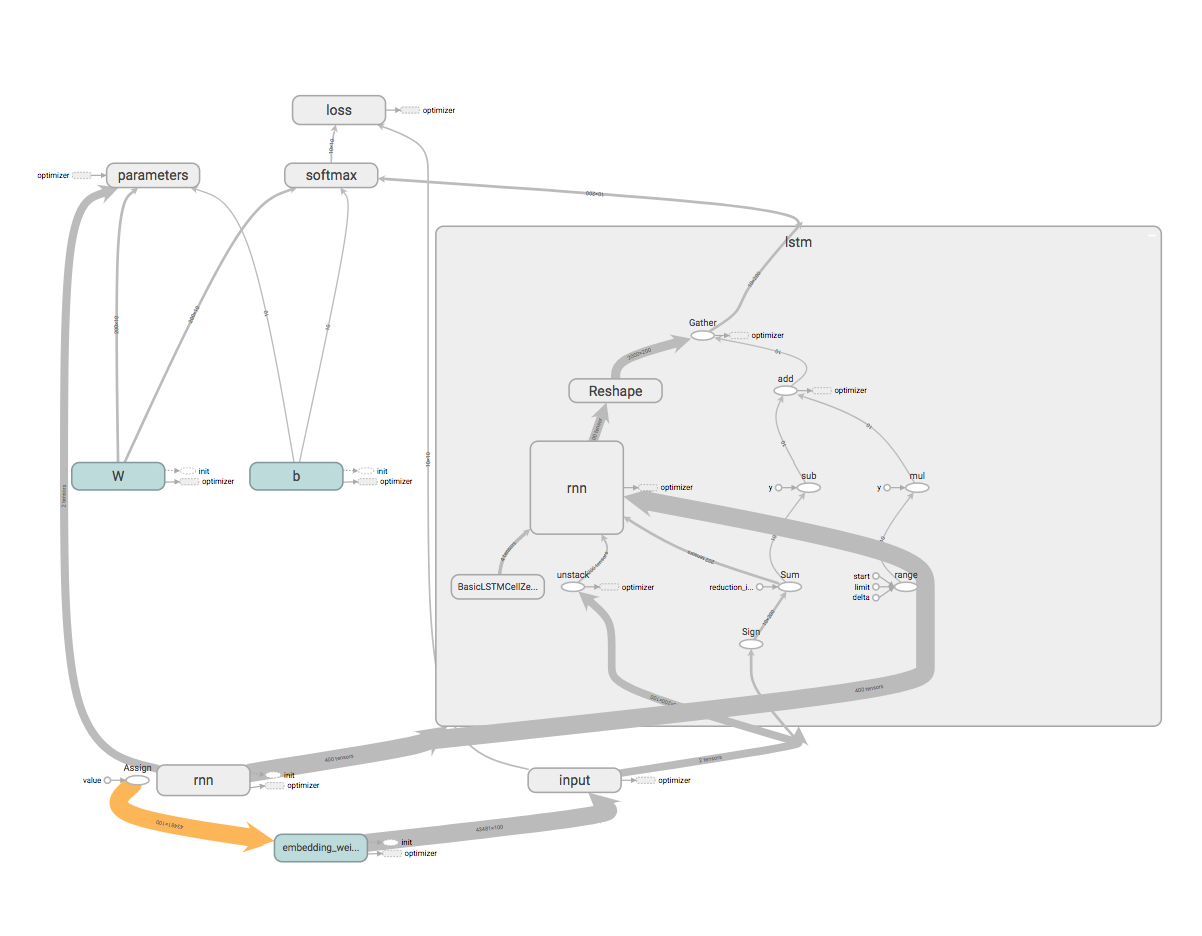
\includegraphics[width=0.45\textwidth]{figure/lstm_architecture}
        \caption{Our LSTM architecture visualized with Tensorboard.}
    \end{figure}

\subsubsection{Convolutional Neural Network}
\label{model:back:cnn}
    CNN uses multiple layers of convolving filters that apply on the input data and
    calculate the output after all feeding the input through all of the layers. Although
    originally built for computer vision, CNNs have shown quite significant potential in
    natural language processing (NLP), and especially in sentence classification.
    Our chosen network architecture is based upon Yoon Kim's work on sentence
    classification\cite{kim2014convolutional}. The architecture consists of four 
    main parts: a word
    embedding layer, a convolution layer, a pooling layer and a fully connected layer
    at the end.
    \begin{figure*}
    \center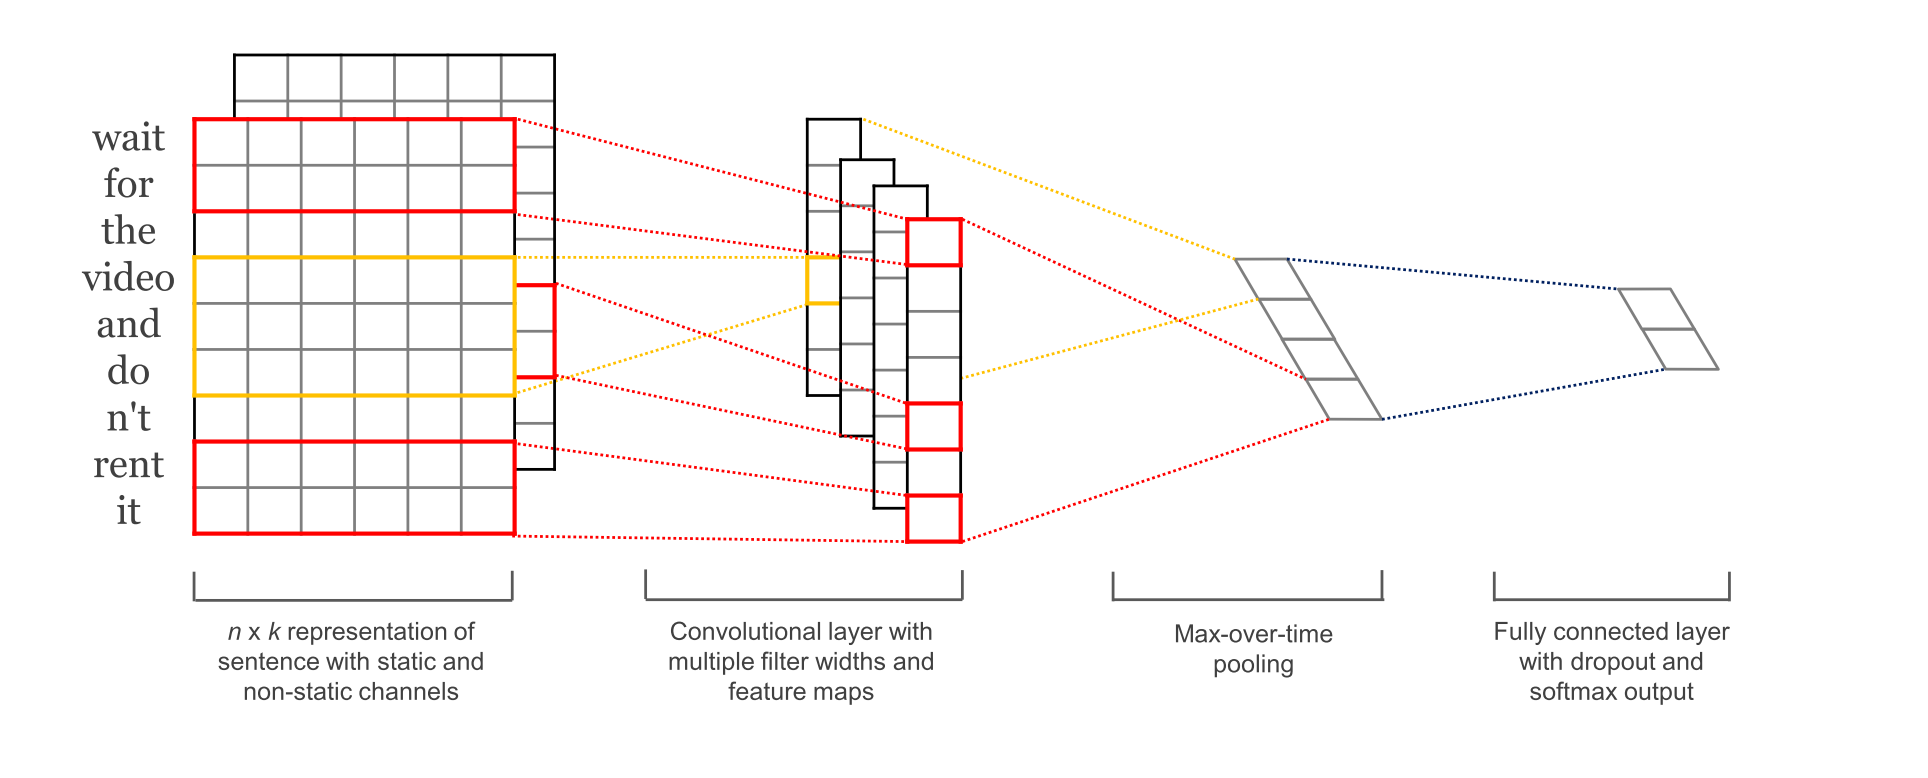
\includegraphics[width=0.9\textwidth]{figure/sc_model}
    \caption{Model architecture with two channels for an example sentence,
     figure credit: \cite{kim2014convolutional}}
    \end{figure*}

    As with the LSTM model, distributed word embeddings allow us to represent a 
    word as a vector in multi-dimensional space, and they form the basis for feeding 
    text into the deep learning model. However, instead of feeding word vectors into
    our model one-by-one, we concatenate our word vectors together into a fixed-length
    input vector which we convolve over to create feature maps. 

    Let $x_{i} \in \mathbb{R}^k$ be a dimentional word vector representing the $i$-th word in the
    sentence. Thus, the sentence would be represented by
    \begin{equation}
    x_{1:n} = x_1 \oplus x_2 \oplus ... \oplus x_n
    \end{equation}
    $\oplus$ signifies concatenation. Suppose $x_{i:i+j}$ refers to concatenating
    word vectors $x_i, x_{i+1}, ... , x_{i+j}$. The convolution operator with a filter
    $W \in \mathbb{R}^{hk}$ applied to a window size of $h$
    words is defined as
    \begin{equation}
    c_i = f(W \cdot x_{i:i_{h-1}} + b)
    \end{equation}
    $b$ is a bias term and $f$ signifies a non linear function such as the hyperbolic
    tangent. We use this filter to generate a feature map $c = [c_1, c_2, ... ,x_{n-h+1}]$
    with $c \in \mathbb{R}^{n-h+1}$ by applying the filter to each possible window of words in
    the sentence $x_{1:h}, x_{2:h+1}, ... ,x_{n-h+1:n}$.

    We plan to use multiple filters with varying window sizes to obtain multiple features, and we will
    compare our results for different hyperparameters.
    A max-over-time pooling operation $\hat{c}$ = max\{$c$\} will be applied once the feature
    maps are generated. The pooling operation outputs the largest value from each individual
    feature maps. We will employ dropout on the penultimate layer $z = [\hat{c}_1,...,\hat{c}_m]$
    (we have $m$ filters) for regularization with a constraint on $l_2$-norms of the weight
    vectors. This should help prevent co-adaptation of hidden units by randomly setting weights
    to zero for selected neurons. The function is expressed below:

    \begin{equation}
    y = W \cdot (z \circ r) + b
    \end{equation}

    $\circ$ is the element-wise multiplication operator and $r \in \mathbb{R}^m$ is
    the masking vector of Bernoulli random variables with probability $p$ of being 1.
    The gradients are backpropagated through the unmasked units during training. At test
    time, the learned weight vectors are scaled by $p$ such that $\hat{w} = pw$ and $\hat{w}$
    is used to score unseen sentences. Finally, we will constrain $l_2$-norms of the weight
    vectors by rescaling $w$ to have $||w||_2 = s$ whenever $||w||_2 > s$ after a gradient
    decent step.
    
    Due to the strict limitation of man-power and time, we didn't have chance to 
    implement the CNN and compare it with other implementations.

\subsection{Dataset Preprocessing}
    Evaluating both sequential and non-sequential models required our data to be inputted
    in different ways to our Logistic Regression model. To train our baseline logistic regression
    model, we used the tensorflow Dataset API to extract preprocessed word counts for each
    review from from a feature file prepared by \cite{maas2011learning}. Due to the linearity of
    the logistic regression model and the Zipf distribution of word frequencies, we chose
    to ignore the word counts and instead use binary features.
    
    When training the LSTM, we set the max size of our reviews at 200 tokens to ease
    computation constraints. Reviews of excess length were truncated, and shorter reviews 
    were padded with zeros. Word tokenization was preformed using the nltk python library,
    which uses a custom version of the Stanford Treebank tokenizer. In addition, we separated
    periods, quotation marks, dashes, and slashes into their own tokens, so that the LSTM 
    would be able to learn how to generalize about their functionality. Treating dashes as tokens,
    for instance will often reduce the size of the model vocabulary, since words such as
     "broken-hearted" can be decomposed into three tokens: "broken", "-", and "hearted".
     
    In addition, we attempted to ameliorate the problem of zero-shot earning by removing 
    infrequently occurring words from our vocabulary. We replaced the bottom-$k$ 
    least-frequently occurring words with an $<UNK>$ token, which the model could then
    learn to represent any out-of-vocabulary term. Since the Zipf distribution of word frequencies
    means that most text content is composed of a small number of different words, removing all
    single-occurrence words from our dataset modified less than 0.75\% of the training dataset.
     
    We trained two different LSTM models based on the above preprocessing methods.
    ``LSTM larger'' tokenized lowercase sentences using the nltk tokenizer and had a
    vocabulary size of 87798. "LSTM smaller" used the more aggressive punctuation tokenization
    described above and removed words that had only occurred in the truncated reviews once
    for a total vocabulary size of 43481.

   
\subsection{Network Training}
The results reported
    above were achieved training our model with a 20 shuffled epochs, a
    batch size of 50, a learning rate of \num{1e-4}, and the Adam optimizer.
    In the binomial case, our model is given training data w samples are
    labeled only as positive (the rating is $\leq 5$) or negative (the rating is
    $\geq 6$), and the ground truth score is hidden. We found that this slightly
    increased our accuracy compared to predicting scores from 1-10 and
    bucketing the scores afterwards. In the multinomial case, our model is
    shown the complete rating and predicts scores from 1-10.



    The LSTM was trained using the Adam optimizer and a learning rate of $\num{1e-3}$. We used a
    validation set of size 2,500 for early stopping and saved the weights every 5000 steps. Each
    batch consisted of a single training sample. All of our experiments with minibatch training 
    quickly converged to a local minimum far from the global optimum. Our model scored highest 
    on the validation set after two epochs of training, and we used those weights to score the test set.
    
    When we experimented with very large numbers of weights (removing no words from the 
    vocabulary and using a worse tokenization function gave us a vocabulary of over 87,000),
    our LSTM model had difficulty learning and, possibly due to parameter instability, would start
    outputting NaN loss after approximately one epoch of training. To help stabilize the weights,
    we added an L2 normalization of $1\time10^{-5}$ to our cost functions. While this enabled us
    to train our model, it trained slower and had poorer results compared with our reduced vocabulary 
    LSTM.

\subsection{Front End}
\label{model:front}
    
    The system architecture described in \autoref{model:back} enlaces up to decide the
    sentiment of movie reviews on command line interface. But since a trained network can
    decide the sentiment of input review in a reasonably short period of time. We also
    to build the front end of the system, so people can use the system by visiting a
    url from web browser.
    
\subsubsection{Web Interface by Python \& Flask}
\label{model:front:web}
    Our project is written in Python, so it is only natural to think the web interface =
    should also be build with web frameworks in Python environments. 
    In this project, the web interface it done by the Micro-framework for 
    Python called Flask\cite{ronacher2010flask,grinberg2018flask}.
    
    The web interface contains a page for data input/model selection 
    (\autoref{fig:flask_in}) and another page for
    showing results (\autoref{fig:flask_out}).
    
    \begin{figure}
        \center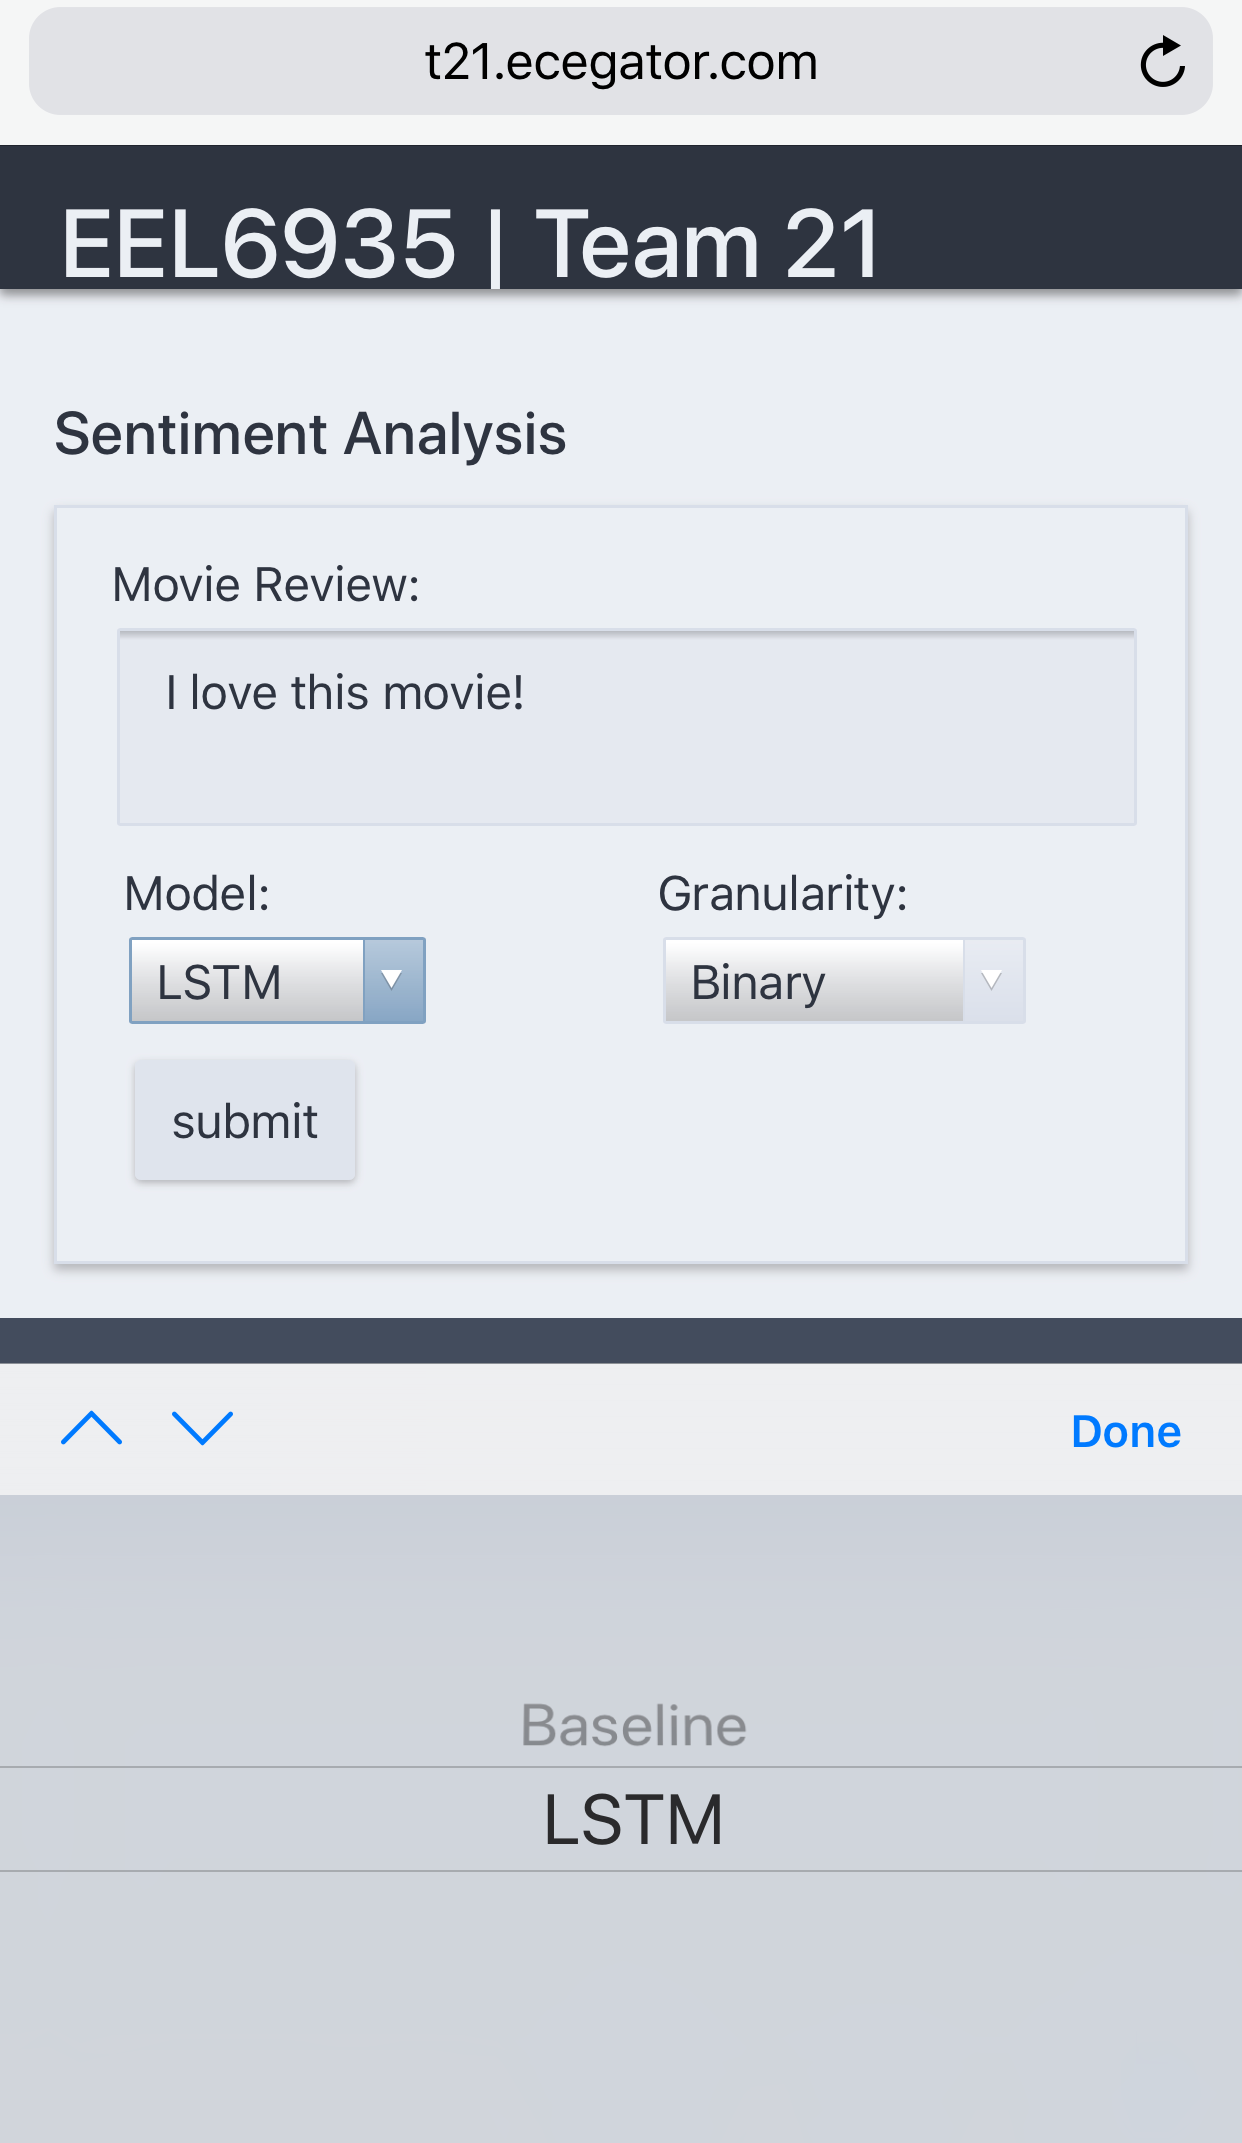
\includegraphics[width=0.4\textwidth]{figure/flask_input}
        \caption{Page for data input and model selection. Both baseline model (logistic
        regression) and LSTM model can be selected. And output can be set to be binary 
        or multi-level}
        \label{fig:flask_in}
    \end{figure}
    
    \begin{figure}
        \center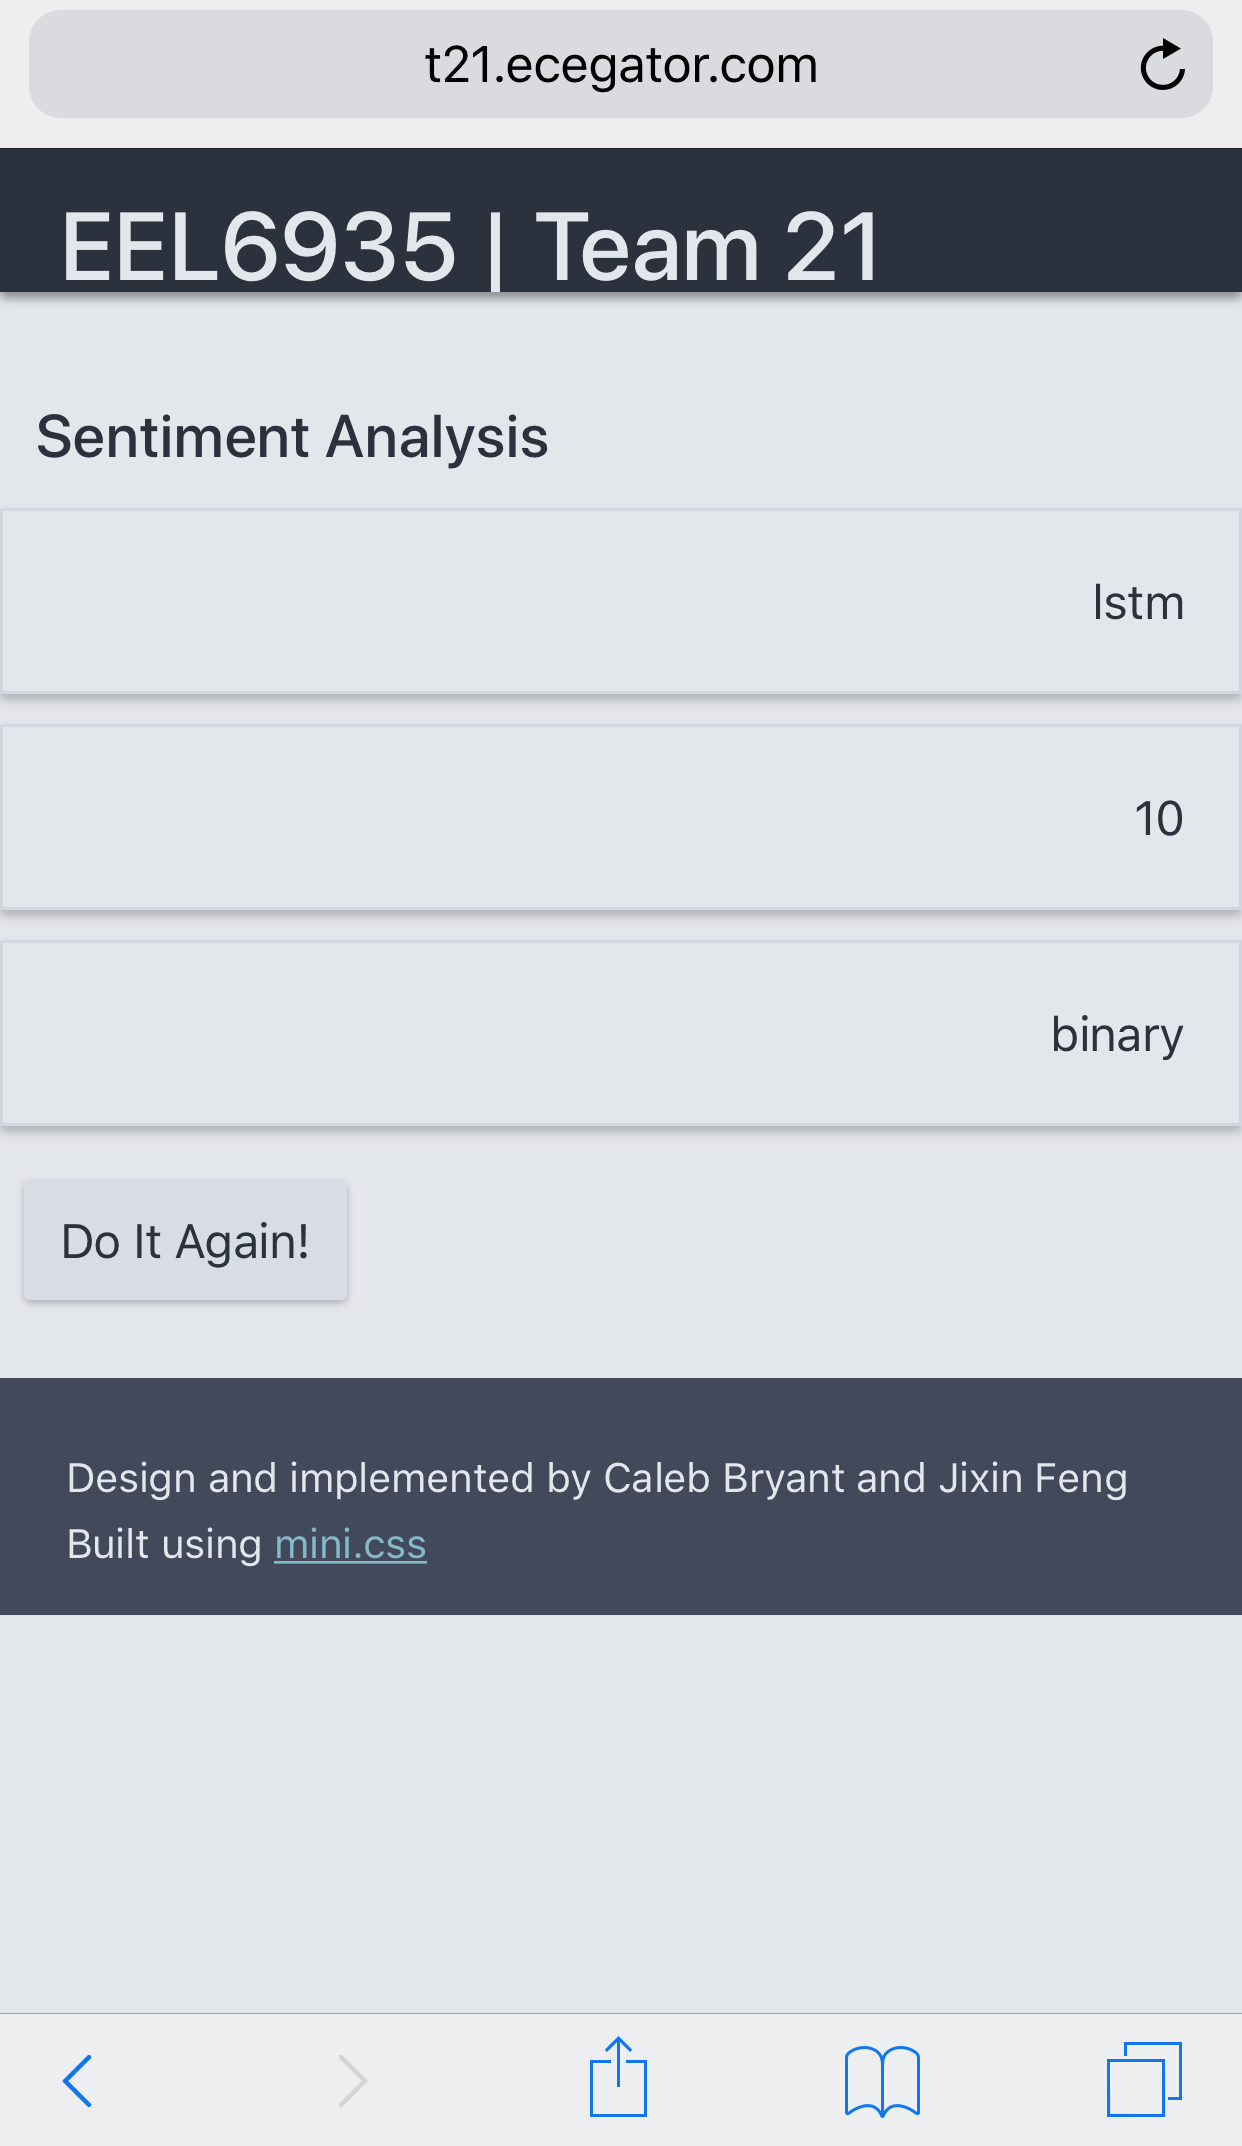
\includegraphics[width=0.4\textwidth]{figure/flask_output}
        \caption{Page for data output, the model selected, output scale and
        sentiment analysis score are shown in a table}
        \label{fig:flask_out}
    \end{figure}
    
\subsubsection{Web Hosting}
\label{model:front:host}
    The Flask powered web app need be hosted in order to be accessed. For security concern,
    we decided to host the app on a Ubuntu 16.04 LTS based virtual machine with 2GB ram and
    1 CPU core. We also registered the domain name: \url{t21.ecegator.com} and generated
    QR code shown in \autoref{fig:qr}
    \begin{figure}
        \center
\includegraphics[width=0.15\textwidth]{figure/qr_website}
        \caption{QR code to access our web app at \url{t21.ecegator.com}}
        \label{fig:qr}
    \end{figure}
    Due to the limitation of our server resources, the web app may not be kept online
    all the time, but we will try our best to keep it running during our presentation
    and the workshop.

\section{Performance Evaluation}
\label{performance}
    \begin{table*}[]
        \centering
        \caption{Sentiment Analysis Result Comparison}
        \label{my-label}
        \begin{tabularx}{\textwidth}{ X X X  X X  X }
        \toprule
        Method & Epochs & Binomial Training & Binomial Testing & Multinomial Training & Multinomial Testing \\
        \midrule
        scikit-learn LR & N/A & 0.9981 & \textbf{0.8697} & N/A & N/A \\
        tensorflow LR & 20 &  0.8670 & 0.8583 & 0.9982 & 0.3734 \\
        larger LSTM & 8 & N/A & N/A & 0.6693 & 0.3657 \\
        smaller LSTM  & 2 & N/A    & 0.8507 & 0.5622   & \textbf{0.4098} \\
        \bottomrule
        \end{tabularx}
    \end{table*}
\subsection{Experiment Setup}
    In order to evaluate our baseline sentiment analysis model, we used the
    Stanford Large Movie Review data set \cite{maas2011learning}. This data
    set consists of 50,000 movie reviews and corresponding scores from IMDb.
    25,000 reviews are designated for training, and 25,000 reviews are designated for testing.
    Each movie rating is an integer between 1 and 10, but the reviews with a rating
    of 5 or 6 were excluded from the dataset
    
    Using this dataset, we preform
    two different machine learning tasks. First, we predict whether a movie review
    has a mostly positive or mostly negative attitude towards the movie of interest. 
    Second, we predict the score of unlabeled movie reviews from 1-10.
    
    Logistic regression models were trained separately for binomial and multinomial
    prediction. Since the LSTM models were  only trained 
    for multinomial classification, predictions were thresholded for binomial 
    classification, and accuracy would likely be improved if the model was modified
    for 2-class classification.
    
    The whole project was coded with python 3, and our evaluation was conducted on
    a Ubuntu 14.04 LTS machine with a 3.1GHz Intel Core i7 CPU with 8MB cache,
    6GB RAM, and a 4GB nVidia GTX 1050 GPU.
    
\subsection{Performance Metrics}
    To measure the performance of our systems, we calculate the raw accuracy
    scores of the systems. We divide the number of correct class predictions
    by the total number of predictions made. Accuracies were calculated
    for both the training and testing sets of the Stanford Large Movie Review dataset.
    
\subsection{Experiment Results}
    In Table 1 we provide the results for our baseline bag of words model using
    two different machine learning toolkits, as well as our two different LSTM models
    
    For the BoW models, the first set of results come from
    using the python scikit-learn package's built in logistic regression model.
    This model relies on highly optimized logistic regression algorithms
    contained in the liblinear \cite{Fan:2008:LLL:1390681.1442794} package,
    and it quickly converged to the global minimum. Since logistic regression
    can be treated as convex optimization problem, we do not have to worry 
    about escaping local optima. We also evaluated the logistic regression
    model using a custom tensorflow implementation. 
        
    While the scikit-learn package included a highly optimized algorithm for
    preforming binomial linear regression, none of the included solvers were
    capable of handling the multinomial linear regression problem due to intensive
    memory usage. Thus we have only provided results from our tensorflow
    model in the multinomial case.
    
    For the LSTM models, we see that having too many parameters in the 
    embedding matrix can have a negative impact on our model's accuracy,
    even though many of the weights were initialized with GloVe embeddings.
    
    \begin{figure}
        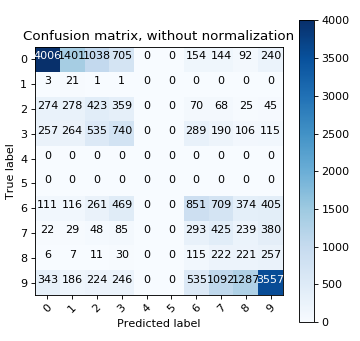
\includegraphics[width=0.45\textwidth]{figure/conf_matrix}
        \caption{The confusion matrix for our LSTM model}
    \end{figure}
    
\section{Conclusion}
\label{conclusion}
    The result shows that the proposed machine learning systems are able to 
    analyze the sentiment of movie reviews generated by human with reasonable
    accuracy. The baseline performance result generated by our Logistic Regression
    model shows that with only conventional machine learning techniques, we can 
    build a good system in short period of time, which is very useful in the
    proof-of-concept stage of system design and system prototyping.
    
    Our LSTM model was able to increase the results of our Logistic Regression model
    by approximately 3\%, which is in line with previous benchmarking by \cite{W17-5202}.
    While Deep Learning has shown impressive results for Computer Vision problems,
    there is still significant room for improvement with NLP problems. Based on our confusion
    matrix, we see that our models still have difficulty determining when some reviews are
    negative and positive, and the model tends to overestimate scores of 1 and 10 -- though
    this is likely the result of the IMDb dataset being unbalanced. It would be useful to 
    have humans label reviews with scores in order to measure how close the models 
    are to achieving human-level accuracy.
        
\section{Future Work}
\label{future}
    Sentiment analysis is a problem which can be studied from multiple angles. But due 
    to the time and man-power limitation, we only compared two different approaches:
    logistic regression and LSTM. In the future, we can try to implement more models used
    for sentiment analysis and compare the complexity, prediction accuracy and other
    system performances. Those system includes Recurrent Convolutional
    Neural Networks (RCNN)\cite{lai2015recurrent}, Very Deep Convolutional Networks 
    (VDCN)\cite{conneau2017very}, etc.
    
    And we only used one deep learning framework in this project. In the future, we
    also aim to learn to use more frameworks like Keras\cite{chollet2015keras},
    Caffe\cite{jia2014caffe}, PyTorch\cite{paszke2017automatic}, 
    Deeplearning4j\cite{nicholson2017deeplearning4j}, etc.
    
    Deep learning has been one of the fastest growing research field sin the history.
    And it shows that science, engineering, biology and art can collaborate together
    in such an elegant way. We believe there must be numerous potential research opportunities
    we can grasp in the future.


\section{Team Coordination}
\label{team}
    This project is done by Caleb Bryant from the CISE department and Jixin Feng from the ECE 
    department. Most machine learning related program including both Logistic 
    Regression and LSTM part are coded by Caleb. Jixin coded the Flask based web app
    and Caleb connected both parts together. The domain name and virtual machine hosting
    the web app is maintained by Jixin and reports, slides used for presentation
    is written by both Jixin and Caleb in \LaTeX.
    
    The detailed record of contribution history is maintained in the project Git repository
    \url{https://github.com/ufjfeng/EEL6935-Course-Project} hosted on GitHub.


\bibliographystyle{IEEEtran}
\bibliography{eel6935_final.bib}

\end{document}
